% Entrega A9 — Apresentação do projeto WP1A (SPEC-009 §3.3)
% Síntese de A7/A8; números rastreáveis a results/ (DOC-R03). Experimento: exp-a4-v2.
\documentclass[aspectratio=169,11pt]{beamer}

\usepackage{fontspec}
\usepackage{booktabs}
\usepackage{graphicx}
\usepackage{hyperref}
\usepackage{microtype}

\setmainfont{DejaVu Sans}
\setsansfont{DejaVu Sans}
\setmonofont{DejaVu Sans Mono}

\usetheme{Madrid}
\usecolortheme{default}
\definecolor{WPTeal}{HTML}{0F4C5C}
\definecolor{WPAccent}{HTML}{E36414}
\definecolor{WPMuted}{HTML}{5C6B73}
\setbeamercolor{structure}{fg=WPTeal}
\setbeamercolor{title}{fg=WPTeal}
\setbeamercolor{frametitle}{fg=WPTeal}
\setbeamercolor{button}{bg=WPTeal,fg=white}
\setbeamercolor{block title}{bg=WPTeal,fg=white}
\setbeamercolor{block body}{bg=WPTeal!8}
\setbeamertemplate{navigation symbols}{}
\setbeamertemplate{footline}{%
  \hfill\insertframenumber/\inserttotalframenumber\hspace*{1em}\vspace*{0.4em}%
}

\graphicspath{{../article/figures/}}

\title[WP1A --- Benchmark TEP]{Benchmark reproduzível de métodos clássicos\\
para diagnóstico de falhas no Tennessee Eastman Process}
\subtitle{Entrega A9 --- síntese do relatório técnico (A7) e do manuscrito (A8)}
\author{Grupo A --- WP1A / MEI0028 --- Modelagem e Simulação\\
Pontifícia Universidade Católica de Goiás}
\date{Experimento oficial: \texttt{exp-a4-v2} \quad|\quad 2026-09-14}

\begin{document}

%------------------------------------------------------------------------------
\begin{frame}
\titlepage
\vspace{-0.5em}
\centering
{\scriptsize Números citados $\leftrightarrow$ \texttt{results/} (DOC-R03). Sem causalidade física (INV-08).\\
Sem ``melhor modelo'' por acurácia só (INV-06).}
\end{frame}

%------------------------------------------------------------------------------
\begin{frame}{Agenda}
\tableofcontents
\end{frame}

%==============================================================================
\section{Problema e objetivos}
%==============================================================================
\begin{frame}{Problema}
\begin{itemize}
  \item Diagnóstico multiclasse de falhas no \textbf{Tennessee Eastman Process} (TEP):
        52 variáveis, 21 classes (1 normal + 20 falhas).
  \item Estudos comparativos costumam misturar protocolos, vazar informação temporal
        entre partições e eleger ``vencedor'' só por acurácia.
  \item \textbf{WP1A:} benchmark \emph{reproduzível} de 6 famílias clássicas sob
        protocolo único, multicritério (desempenho + custo).
\end{itemize}
\bigskip
\begin{block}{Objetivo geral}
Comparar Regressão Logística, Árvore, Random Forest, Gradient Boosting, SVM e
XGBoost sem vazamento por execução (\texttt{run}), isolando o teste até o
congelamento das configurações.
\end{block}
\end{frame}

%------------------------------------------------------------------------------
\begin{frame}{Questões de pesquisa (QP1--QP5)}
\begin{enumerate}
  \item[\textbf{QP1}] Quais algoritmos têm melhor desempenho \emph{global}?
  \item[\textbf{QP2}] O ranking é consistente sob equilíbrio entre classes
        (Acc vs BA/F1/MCC)?
  \item[\textbf{QP3}] Quais falhas são sistematicamente mais difíceis?
  \item[\textbf{QP4}] Complexidade justifica maior custo computacional?
  \item[\textbf{QP5}] Qual o melhor \emph{compromisso} desempenho $\times$ tempo $\times$ tamanho?
\end{enumerate}
\end{frame}

%------------------------------------------------------------------------------
\begin{frame}{Hipóteses (H1--H4)}
\begin{description}
  \item[H1] Ensembles em árvore $>$ Regressão Logística (F1 e/ou MCC).
  \item[H2] XGBoost e RF $>$ LR e árvore isolada (F1 e MCC).
  \item[H3] LR competitiva em custo; F1 reduzido nas falhas difíceis.
  \item[H4] Melhor por acurácia $\neq$ melhor por F1 / MCC / custo de inferência.
\end{description}
\bigskip
{\small Critérios binários SPEC-000~\S4: \emph{corroborada} / \emph{refutada}.
Evidência em dois planos: holdout global + testes SPEC-008 por \texttt{run}.}
\end{frame}

%==============================================================================
\section{Protocolo}
%==============================================================================
\begin{frame}{Unidade experimental e anti-vazamento}
\begin{columns}[T]
\begin{column}{0.55\textwidth}
\begin{itemize}
  \item Unidade = \textbf{execução} (\texttt{run\_id}), nunca a amostra (UE-01).
  \item Partições com interseção vazia de runs (INV-01/02).
  \item Scaler \texttt{fit} só no treino (INV-04).
  \item Teste consultado \textbf{uma vez}, após freeze (INV-05).
  \item Mesmo manifesto + preprocessor para os 6 modelos (INV-03).
\end{itemize}
\end{column}
\begin{column}{0.42\textwidth}
\begin{block}{Pipeline}
Audit $\to$ EDA $\to$ Split\\
$\to$ Preprocess $\to$ Train\\
$\to$ Eval $\to$ Stats\\
$\to$ Figures $\to$ Report
\end{block}
{\scriptsize Experimento: \texttt{exp-a4-v2}\\
Semente: 42\\
Dataset: \texttt{tep-canonical-v1}}
\end{column}
\end{columns}
\end{frame}

%------------------------------------------------------------------------------
\begin{frame}{Dados e divisão}
\begin{columns}[T]
\begin{column}{0.48\textwidth}
\begin{tabular}{lr}
\toprule
Item & Valor \\
\midrule
Features & 52 \\
Classes & 21 \\
Runs & 42 \\
Linhas & 30\,260 \\
\bottomrule
\end{tabular}
\bigskip
{\scriptsize Fonte: A6 dataset summary.}
\end{column}
\begin{column}{0.48\textwidth}
\begin{itemize}
  \item Treino: 21 runs\\
        Val: 10 \quad Teste: 11
  \item \textbf{Limitação (AR-1):} com 2 runs/classe,
        classes de val e teste são \emph{disjuntas}.
  \item Scorer de seleção = acurácia na val (AR-2).
  \item Grids desiguais nesta baseline (AR-3).
\end{itemize}
\end{column}
\end{columns}
\end{frame}

%==============================================================================
\section{Resultados}
%==============================================================================
\begin{frame}{Métricas globais no teste (A5)}
{\small
\begin{tabular}{lrrrrr}
\toprule
Modelo & Acc & BA & F1$_m$ & MCC & Treino\,s \\
\midrule
Reg.\ logística & 0,275 & 0,164 & 0,184 & 0,250 & 3,7 \\
Árvore & 0,564 & 0,303 & 0,314 & 0,560 & 1,4 \\
Random forest & 0,617 & \textbf{0,333} & \textbf{0,357} & \textbf{0,597} & 3,1 \\
Grad.\ boosting & 0,608 & 0,321 & 0,347 & 0,584 & 282 \\
SVM linear & 0,237 & 0,150 & 0,163 & 0,215 & 177 \\
XGBoost & \textbf{0,618} & 0,330 & 0,353 & 0,596 & 22 \\
\bottomrule
\end{tabular}
}
\bigskip
{\scriptsize Fonte: \texttt{A5\_exp-a4-v2\_\_global\_metrics.csv}. Macro com $C{=}21$
inclui classes ausentes no teste (AR-4).}
\end{frame}

%------------------------------------------------------------------------------
\begin{frame}{F1 macro e MCC}
\begin{center}
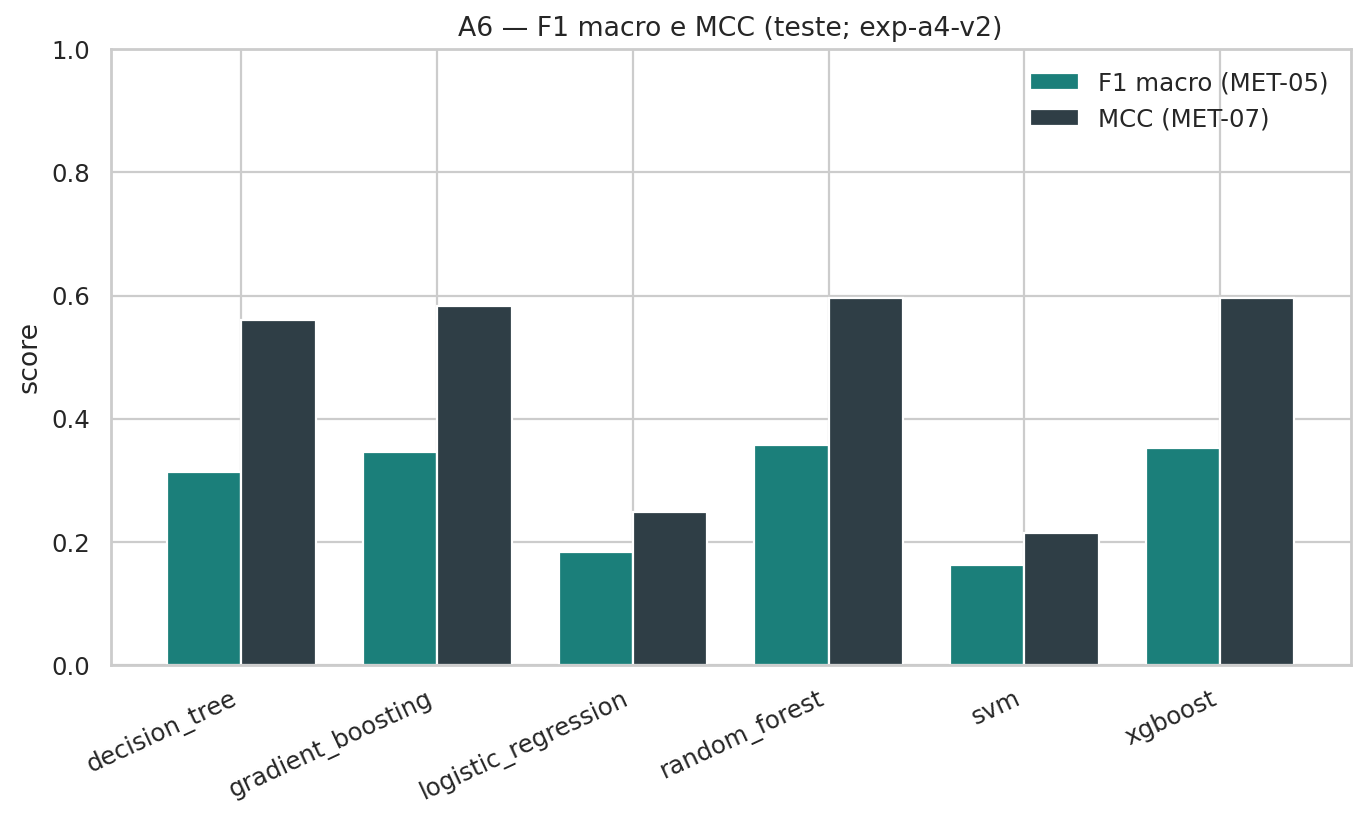
\includegraphics[width=0.88\textwidth]{A6_exp-a4-v2__06_f1_mcc.png}
\end{center}
{\scriptsize Figura A6 --- \texttt{article/figures/A6\_exp-a4-v2\_\_06\_f1\_mcc.png}}
\end{frame}

%------------------------------------------------------------------------------
\begin{frame}{Custo computacional}
\begin{center}
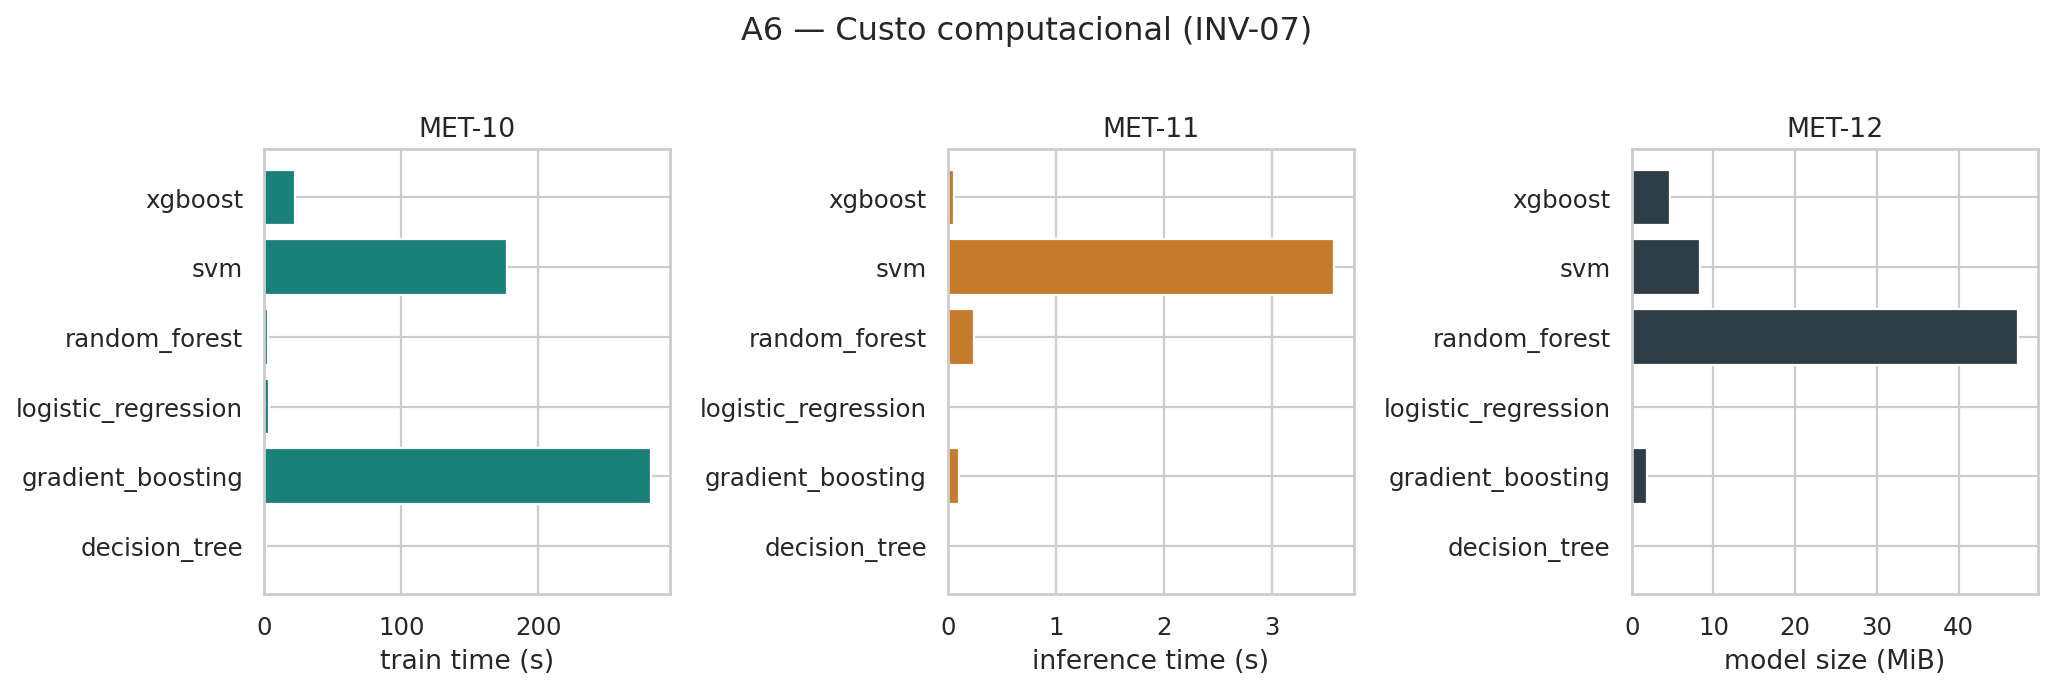
\includegraphics[width=0.88\textwidth]{A6_exp-a4-v2__07_computational_cost.png}
\end{center}
{\scriptsize Figura A6 --- custo (treino, inferência, tamanho). INV-07.}
\end{frame}

%------------------------------------------------------------------------------
\begin{frame}{Respostas a QP1--QP5 (síntese)}
\begin{description}
  \item[QP1] Grupo superior: RF, XGB, GB; inferior: LR, SVM linear.
  \item[QP2] Ranking Acc (XGB$\to$RF) $\neq$ BA/F1/MCC (RF$\to$XGB).
  \item[QP3] Classes presentes mais difíceis: \textbf{3, 15, 10};
        confusões 10$\to$15 e 3$\to$15 (sem causalidade física).
  \item[QP4] GB (treino $\approx$282\,s) não supera RF/XGB; SVM linear caro e fraco.
  \item[QP5] RF (F1/MCC); XGB (compromisso); DT (custo mínimo) --- sem vencedor único.
\end{description}
\end{frame}

%------------------------------------------------------------------------------
\begin{frame}{Estatística formal (SPEC-008)}
\begin{itemize}
  \item Unidade = \texttt{run\_id}; $n{=}11$ runs de teste; métrica = \texttt{run\_accuracy}.
  \item \textbf{Friedman:} $\chi^2{=}14{,}08$, $p{=}0{,}015$ --- rejeita igualdade global.
  \item \textbf{Wilcoxon + Holm} (famílias planejadas):
  \begin{itemize}
    \item H1 (3 pares vs LR): \textbf{corroborada} em run-level.
    \item H2 (4 pares vs LR/DT): \textbf{não corroborada} (nenhum par após Holm; AR-5).
  \end{itemize}
\end{itemize}
\begin{block}{Dois planos de evidência}
§4 (F1/MCC/custo globais) \quad\textit{e}\quad SPEC-008 (\texttt{run\_accuracy}).
Concordância não é automática.
\end{block}
\end{frame}

%------------------------------------------------------------------------------
\begin{frame}{Vereditos H1--H4}
{\small
\begin{tabular}{lll}
\toprule
H & Holdout (§4) & Run-level (SPEC-008) \\
\midrule
H1 & \textbf{Corroborada} & \textbf{Corroborada} (Holm, fam.\ 3) \\
H2 & \textbf{Corroborada} & \textbf{Não corroborada} (fam.\ 4) \\
H3 & \textbf{Corroborada} & N/A (critério custo/F1 classe) \\
H4 & \textbf{Corroborada} & N/A (multicritério) \\
\bottomrule
\end{tabular}
}
\bigskip
\begin{itemize}
  \item H4: líderes distintos --- XGB (Acc), RF (F1/MCC), DT (inferência).
  \item Sem interpretação causal de atributos (INV-08).
\end{itemize}
\end{frame}

%==============================================================================
\section{Ameaças e conclusões}
%==============================================================================
\begin{frame}{Ameaças / riscos aceitos (AR-1--AR-5)}
\begin{itemize}
  \item \textbf{AR-1} Classes val $\cap$ teste $= \emptyset$ (2 runs/classe).
  \item \textbf{AR-2} Scorer de seleção = acurácia amostral.
  \item \textbf{AR-3} Orçamentos de busca desiguais; SVM só linear.
  \item \textbf{AR-4} Macro $C{=}21$ com $\sim$10 classes ausentes no teste.
  \item \textbf{AR-5} Semente única; $n{=}11$ (baixo poder).
\end{itemize}
\bigskip
{\small Formalizados na revisão
\texttt{A8\_scientific\_review\_exp-a4-v3\_post\_remediation.md}:
\textbf{APPROVE WITH ACCEPTED RISKS}. Protocolo congelado --- remoção exige novo
\texttt{experiment\_id}.}
\end{frame}

%------------------------------------------------------------------------------
\begin{frame}{Conclusões}
\begin{enumerate}
  \item Benchmark ponta a ponta com anti-vazamento por \texttt{run} e avaliação multicritério.
  \item RF/XGB/GB lideram; LR e SVM linear atrás; \textbf{não} há único melhor modelo.
  \item H1--H4 \emph{corroboradas} em §4; H1 também em run-level; H2 não (poder / família Holm).
  \item Compromisso observacional: \textbf{XGBoost}; pico F1/MCC: \textbf{RF}; custo mínimo: \textbf{DT}.
  \item Referência clássica para trabalhos futuros (profundos, físico-informados, detecção precoce),
        sob AR-1--AR-5.
\end{enumerate}
\end{frame}

%------------------------------------------------------------------------------
\begin{frame}{Artefatos e rastreabilidade}
\begin{itemize}
  \item A5 métricas: \texttt{results/tables/A5\_exp-a4-v2\_\_*}
  \item A6 figuras: \texttt{article/figures/A6\_exp-a4-v2\_\_*}
  \item SPEC-008: \texttt{results/tables/A8\_exp-a4-v2\_\_*} /
        \texttt{results/metrics/A8\_exp-a4-v2\_\_statistics.json}
  \item A7: \texttt{reports/technical/A7\_technical\_report.pdf}
  \item A8: \texttt{article/manuscript/manuscript.pdf}
  \item Revisão: \texttt{A8\_scientific\_review\_exp-a4-v3\_post\_remediation.md}
\end{itemize}
\bigskip
\begin{center}
\textbf{Obrigado}\\[0.5em]
{\small Grupo A --- WP1A / MEI0028}
\end{center}
\end{frame}

\end{document}
